\documentclass{standalone}
\usepackage{tikz}
\usepackage{hyperref}
\usepackage{dictsym}

\usetikzlibrary{shadows,calc,math,shadings}


\newcommand{\html}[2]{\href{../html/#1/explanations.html}{#2}}
\newcommand{\mathy}{\dsmathematical}


\begin{document}

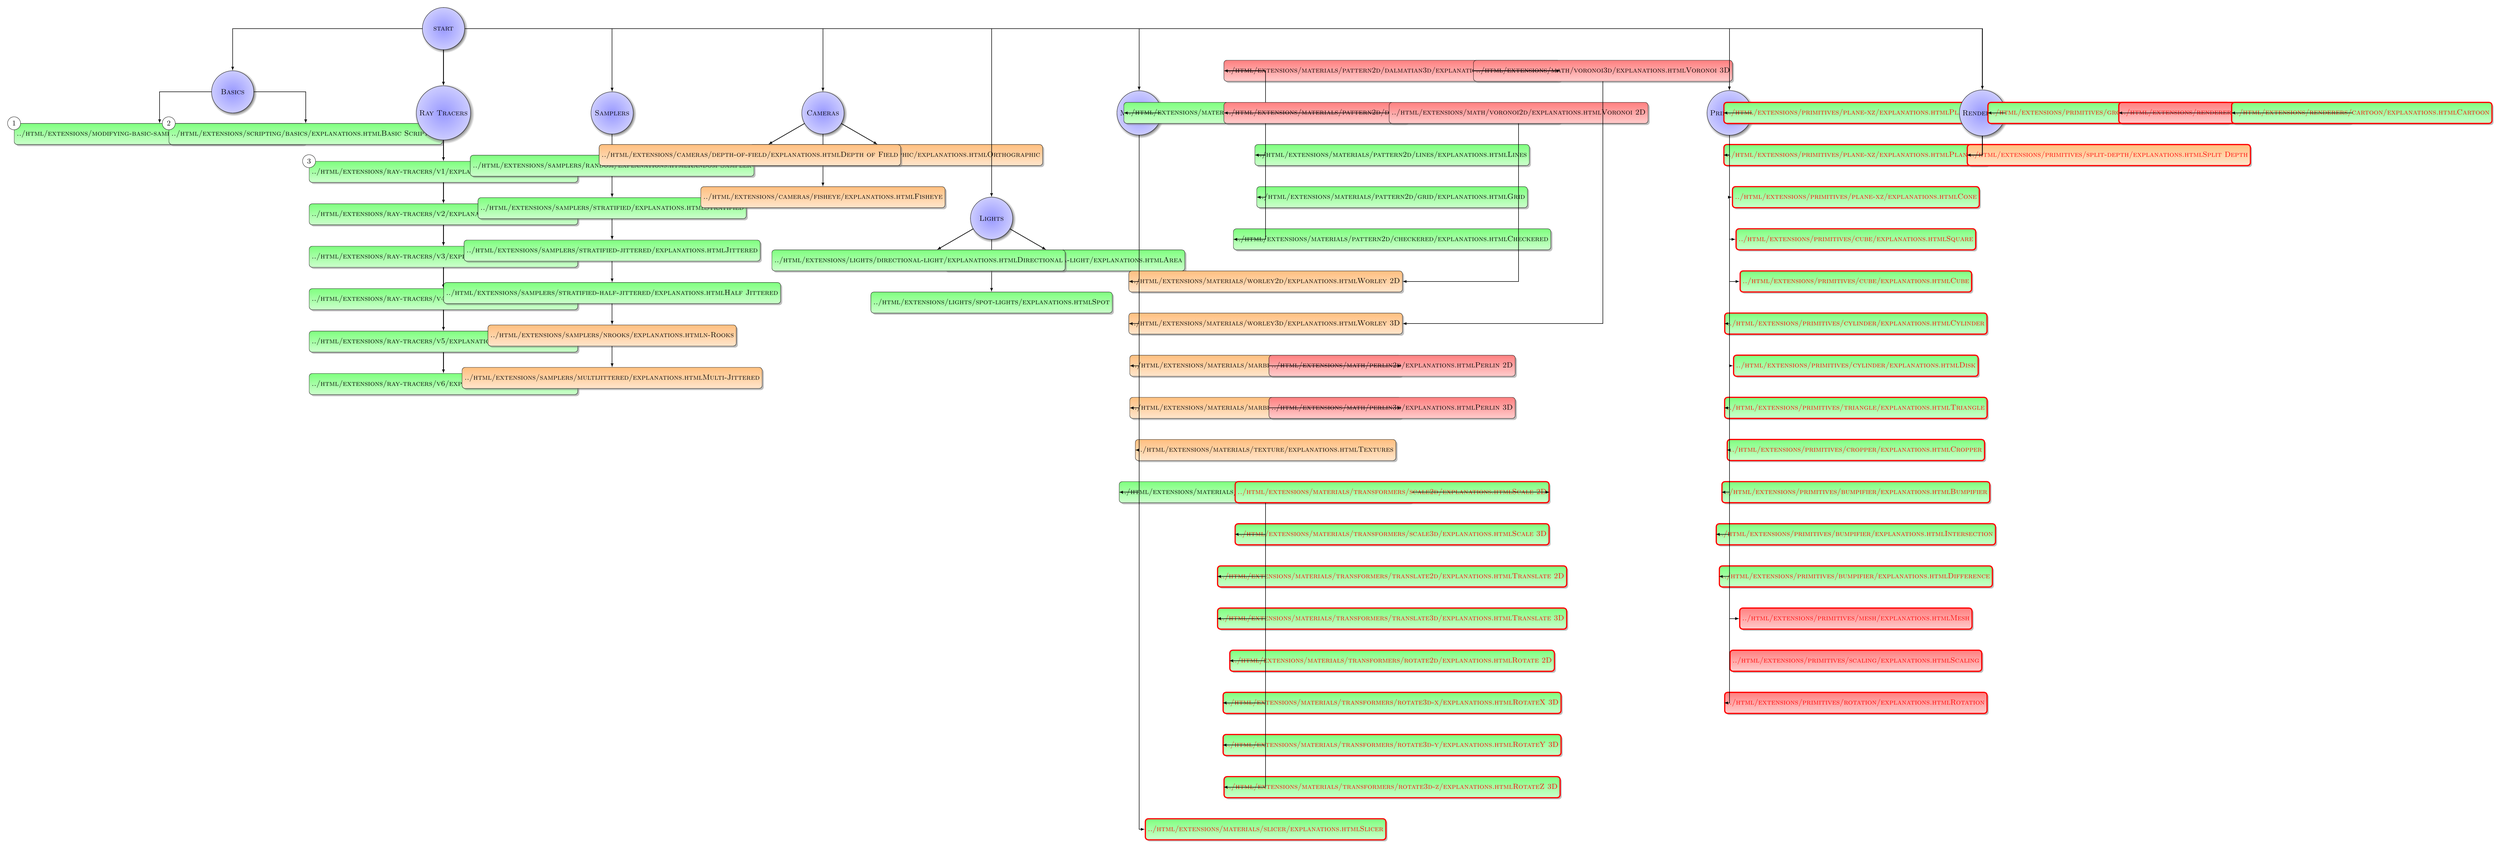
\begin{tikzpicture}[extension/.style={draw,minimum width=5cm,minimum height=1cm,font=\scshape,rounded corners=4pt,drop shadow},
                    dependency/.style={thick,latex-},
                    node/.style={circle,draw,shading=radial,minimum size=2cm,inner color=blue!40,outer color=blue!20,font=\scshape,circular drop shadow},
                    area/.style={left color=gray!30,right color=gray!10,rounded corners=4pt},
                    easy/.style={top color=green!50,bottom color=green!20},
                    medium/.style={top color=orange!50,bottom color=orange!20},
                    hard/.style={top color=red!50,bottom color=red!20},
                    order/.style={draw,circle,fill=white},
                    todo/.style={red,ultra thick}]
  \pgfdeclarelayer{background}
  \pgfdeclarelayer{foreground}
  \pgfsetlayers{background,main,foreground}

  \begin{pgfonlayer}{main}
    \node[node] (start) {start};

    \node[node] (basics) at ($ (start) + (-10, -3) $) {Basics};
    \draw[dependency] (basics) |- (start);

    \node[extension,easy] (modifying basic sample) at ($ (basics) + (-150:4) $) {\html{extensions/modifying-basic-sample}{Basic Sample}};
    \draw[dependency] (modifying basic sample) |- (basics);

    \node[extension,easy] (scripting basics) at ($ (basics) + (-30:4) $) {\html{extensions/scripting/basics}{Basic Scripting}};
    \draw[dependency] (scripting basics) |- (basics);

    \node[node] (ray tracers) at ($ (start) + (0,-4) $) {Ray Tracers};
    \draw[dependency] (ray tracers) -- (start);

    \node[extension,anchor=north,easy] (ray tracer v1) at ($ (ray tracers.south) + (0,-1) $) {\html{extensions/ray-tracers/v1}{Ray Tracer v1}};
    \draw[dependency] (ray tracer v1) -- (ray tracers);

    \node[extension,anchor=north,easy] (ray tracer v2) at ($ (ray tracer v1.south) + (0,-1) $) {\html{extensions/ray-tracers/v2}{Ray Tracer v2}};
    \draw[dependency] (ray tracer v2) -- (ray tracer v1);

    \node[extension,anchor=north,easy] (ray tracer v3) at ($ (ray tracer v2.south) + (0,-1) $) {\html{extensions/ray-tracers/v3}{Ray Tracer v3}};
    \draw[dependency] (ray tracer v3) -- (ray tracer v2);

    \node[extension,anchor=north,easy] (ray tracer v4) at ($ (ray tracer v3.south) + (0,-1) $) {\html{extensions/ray-tracers/v4}{Ray Tracer v4}};
    \draw[dependency] (ray tracer v4) -- (ray tracer v3);

    \node[extension,anchor=north,easy] (ray tracer v5) at ($ (ray tracer v4.south) + (0,-1) $) {\html{extensions/ray-tracers/v5}{Ray Tracer v5}};
    \draw[dependency] (ray tracer v5) -- (ray tracer v4);

    \node[extension,anchor=north,easy] (ray tracer v6) at ($ (ray tracer v5.south) + (0,-1) $) {\html{extensions/ray-tracers/v6}{Ray Tracer v6}};
    \draw[dependency] (ray tracer v6) -- (ray tracer v5);

    \node[node] (samplers) at ($ (ray tracers) + (8,0) $) {Samplers};
    \draw[dependency] (samplers) |- (start);

    \node[extension,anchor=north,easy] (random sampler) at ($ (samplers) + (0,-2) $) {\html{extensions/samplers/random}{Random Sampler}};
    \draw[dependency] (random sampler) -- (samplers);

    \node[extension,anchor=north,easy] (stratified sampler) at ($ (random sampler.south) + (0,-1) $) {\html{extensions/samplers/stratified}{Stratified}};
    \draw[dependency] (stratified sampler) -- (random sampler);

    \node[extension,anchor=north,easy] (jittered sampler) at ($ (stratified sampler.south) + (0,-1) $) {\html{extensions/samplers/stratified-jittered}{Jittered}};
    \draw[dependency] (jittered sampler) -- (stratified sampler);

    \node[extension,anchor=north,easy] (half jittered sampler) at ($ (jittered sampler.south) + (0,-1) $) {\html{extensions/samplers/stratified-half-jittered}{Half Jittered}};
    \draw[dependency] (half jittered sampler) -- (jittered sampler);

    \node[extension,anchor=north,medium] (nrooks sampler) at ($ (half jittered sampler.south) + (0,-1) $) {\html{extensions/samplers/nrooks}{n-Rooks}};
    \draw[dependency] (nrooks sampler) -- (half jittered sampler);

    \node[extension,anchor=north,medium] (multijittered sampler) at ($ (nrooks sampler.south) + (0,-1) $) {\html{extensions/samplers/multijittered}{Multi-Jittered}};
    \draw[dependency] (multijittered sampler) -- (nrooks sampler);

    \node[node] (cameras) at ($ (samplers) + (10,0) $) {Cameras};
    \draw[dependency] (cameras) |- (start);

    \node[extension,medium] (orthographic camera) at ($ (cameras) + (-30:4) $) {\html{extensions/cameras/orthographic}{Orthographic}};
    \draw[dependency] (orthographic camera) -- (cameras);

    \node[extension,medium] (fisheye camera) at ($ (cameras) + (-90:4) $) {\html{extensions/cameras/fisheye}{Fisheye}};
    \draw[dependency] (fisheye camera) -- (cameras);

    \node[extension,medium] (depth of field camera) at ($ (cameras) + (-150:4) $) {\html{extensions/cameras/depth-of-field}{Depth of Field}};
    \draw[dependency] (depth of field camera) -- (cameras);

    \node[node] (lights) at ($ (cameras) + (8,-5) $) {Lights};
    \draw[dependency] (lights) |- (start);

    \node[extension,easy] (area light) at ($ (lights) + (-30:4) $) {\html{extensions/lights/area-light}{Area}};
    \draw[dependency] (area light) -- (lights);

    \node[extension,easy] (spot light) at ($ (lights) + (-90:4) $) {\html{extensions/lights/spot-lights}{Spot}};
    \draw[dependency] (spot light) -- (lights);

    \node[extension,easy] (directional light) at ($ (lights) + (-150:4) $) {\html{extensions/lights/directional-light}{Directional}};
    \draw[dependency] (directional light) -- (lights);

    \node[node] (materials) at ($ (cameras) + (15,0) $) {Materials};
    \draw[dependency] (materials) |- (start);

    \node[extension,easy] (pattern 2d materials) at ($ (materials) + (6,0) $) {\html{extensions/materials/patterns2d}{Patterns 2D}};
    \draw[dependency] (pattern 2d materials) -- (materials);

    \node[extension,hard] (dalmatian 2d material) at ($ (pattern 2d materials) + (6,0) $) {\html{extensions/materials/pattern2d/dalmatian2d}{Dalmatian 2D}};
    \draw[dependency] (dalmatian 2d material) -- (pattern 2d materials);

    \node[extension,medium] (worley 2d material) at ($ (materials) + (6,-8) $) {\html{extensions/materials/worley2d}{Worley 2D}};
    \draw[dependency] (worley 2d material) -| (materials);

    \node[extension,hard] (dalmatian 3d material) at ($ (pattern 2d materials) + (6,2) $) {\html{extensions/materials/pattern2d/dalmatian3d}{Dalmatian 3D}};
    \draw[dependency] (dalmatian 3d material) -| (pattern 2d materials);

    \node[extension,medium] (worley 3d material) at ($ (materials) + (6,-10) $) {\html{extensions/materials/worley3d}{Worley 3D}};
    \draw[dependency] (worley 3d material) -| (materials);

    \node[extension,easy] (lines pattern material) at ($ (pattern 2d materials) + (6,-2) $) {\html{extensions/materials/pattern2d/lines}{Lines}};
    \draw[dependency] (lines pattern material) -| (pattern 2d materials);

    \node[extension,easy] (grid pattern material) at ($ (pattern 2d materials) + (6,-4) $) {\html{extensions/materials/pattern2d/grid}{Grid}};
    \draw[dependency] (grid pattern material) -| (pattern 2d materials);

    \node[extension,easy] (checkered pattern material) at ($ (pattern 2d materials) + (6,-6) $) {\html{extensions/materials/pattern2d/checkered}{Checkered}};
    \draw[dependency] (checkered pattern material) -| (pattern 2d materials);

    \node[extension,medium] (marble 2d material) at ($ (materials) + (6,-12) $) {\html{extensions/materials/marble2d}{Marble 2D}};
    \draw[dependency] (marble 2d material) -| (materials);

    \node[extension,medium] (marble 3d material) at ($ (materials) + (6,-14) $) {\html{extensions/materials/marble3d}{Marble 3D}};
    \draw[dependency] (marble 3d material) -| (materials);

    \node[extension,hard] (voronoi 2d) at ($ (dalmatian 2d material) + (6,0) $) {\html{extensions/math/voronoi2d}{Voronoi 2D \mathy}};
    \draw[dependency] (dalmatian 2d material) -- (voronoi 2d);
    \draw[dependency] (worley 2d material) -| (voronoi 2d);

    \node[extension,hard] (voronoi 3d) at ($ (dalmatian 3d material) + (10,0) $) {\html{extensions/math/voronoi3d}{Voronoi 3D \mathy}};
    \draw[dependency] (dalmatian 3d material) -- (voronoi 3d);
    \draw[dependency] (worley 3d material) -| (voronoi 3d);

    \node[extension,hard] (perlin 2d) at ($ (marble 2d material) + (6,0) $) {\html{extensions/math/perlin2d}{Perlin 2D \mathy}};
    \draw[dependency] (marble 2d material) -- (perlin 2d);

    \node[extension,hard] (perlin 3d) at ($ (marble 3d material) + (6,0) $) {\html{extensions/math/perlin3d}{Perlin 3D \mathy}};
    \draw[dependency] (marble 3d material) -- (perlin 3d);

    \node[extension,medium] (texture materials) at ($ (materials) + (6,-16) $) {\html{extensions/materials/texture}{Textures}};
    \draw[dependency] (texture materials) -| (materials);

    \node[extension,easy] (material transformer) at ($ (materials) + (6,-18) $) {\html{extensions/materials/transformer}{Transformer}};
    \draw[dependency] (material transformer) -| (materials);

    \node[extension,easy,todo] (material scale 2d) at ($ (material transformer) + (6,0) $) {\html{extensions/materials/transformers/scale2d}{Scale 2D}};
    \draw[dependency] (material scale 2d) -- (material transformer);

    \node[extension,easy,todo] (material scale 3d) at ($ (material transformer) + (6,-2) $) {\html{extensions/materials/transformers/scale3d}{Scale 3D}};
    \draw[dependency] (material scale 3d) -| (material transformer);

    \node[extension,easy,todo] (material translate 2d) at ($ (material transformer) + (6,-4) $) {\html{extensions/materials/transformers/translate2d}{Translate 2D}};
    \draw[dependency] (material translate 2d) -| (material transformer);

    \node[extension,easy,todo] (material translate 3d) at ($ (material transformer) + (6,-6) $) {\html{extensions/materials/transformers/translate3d}{Translate 3D}};
    \draw[dependency] (material translate 3d) -| (material transformer);

    \node[extension,easy,todo] (material rotate 2d) at ($ (material transformer) + (6,-8) $) {\html{extensions/materials/transformers/rotate2d}{Rotate 2D}};
    \draw[dependency] (material rotate 2d) -| (material transformer);

    \node[extension,easy,todo] (material rotate 3d x) at ($ (material transformer) + (6,-10) $) {\html{extensions/materials/transformers/rotate3d-x}{RotateX 3D}};
    \draw[dependency] (material rotate 3d x) -| (material transformer);

    \node[extension,easy,todo] (material rotate 3d y) at ($ (material transformer) + (6,-12) $) {\html{extensions/materials/transformers/rotate3d-y}{RotateY 3D}};
    \draw[dependency] (material rotate 3d y) -| (material transformer);

    \node[extension,easy,todo] (material rotate 3d z) at ($ (material transformer) + (6,-14) $) {\html{extensions/materials/transformers/rotate3d-z}{RotateZ 3D}};
    \draw[dependency] (material rotate 3d z) -| (material transformer);

    \node[extension,easy,todo] (material slicer) at ($ (materials) + (6,-34) $) {\html{extensions/materials/slicer}{Slicer}};
    \draw[dependency] (material slicer) -| (materials);

    \node[node] (primitives) at ($ (materials) + (28,0) $) {Primitives};
    \draw[dependency] (primitives) |- (start);

    \node[extension,easy,todo] (plane xz) at ($ (primitives) + (6,0) $) {\html{extensions/primitives/plane-xz}{Plane XZ}};
    \draw[dependency] (plane xz) -- (primitives);

    \node[extension,easy,todo] (plane yz) at ($ (primitives) + (6,-2) $) {\html{extensions/primitives/plane-xz}{Plane YZ}};
    \draw[dependency] (plane yz) -| (primitives);

    \node[extension,easy,todo] (cone) at ($ (primitives) + (6,-4) $) {\html{extensions/primitives/plane-xz}{Cone}};
    \draw[dependency] (cone) -| (primitives);

    \node[extension,easy,todo] (square) at ($ (primitives) + (6,-6) $) {\html{extensions/primitives/cube}{Square}};
    \draw[dependency] (square) -| (primitives);

    \node[extension,easy,todo] (cube) at ($ (primitives) + (6,-8) $) {\html{extensions/primitives/cube}{Cube}};
    \draw[dependency] (cube) -| (primitives);

    \node[extension,easy,todo] (cylinder) at ($ (primitives) + (6,-10) $) {\html{extensions/primitives/cylinder}{Cylinder}};
    \draw[dependency] (cylinder) -| (primitives);

    \node[extension,easy,todo] (disk) at ($ (primitives) + (6,-12) $) {\html{extensions/primitives/cylinder}{Disk}};
    \draw[dependency] (disk) -| (primitives);

    \node[extension,easy,todo] (triangle) at ($ (primitives) + (6,-14) $) {\html{extensions/primitives/triangle}{Triangle}};
    \draw[dependency] (triangle) -| (primitives);

    \node[extension,easy,todo] (cropper) at ($ (primitives) + (6,-16) $) {\html{extensions/primitives/cropper}{Cropper}};
    \draw[dependency] (cropper) -| (primitives);

    \node[extension,easy,todo] (bumpifier) at ($ (primitives) + (6,-18) $) {\html{extensions/primitives/bumpifier}{Bumpifier}};
    \draw[dependency] (bumpifier) -| (primitives);

    \node[extension,easy,todo] (intersection) at ($ (primitives) + (6,-20) $) {\html{extensions/primitives/bumpifier}{Intersection}};
    \draw[dependency] (intersection) -| (primitives);

    \node[extension,easy,todo] (difference) at ($ (primitives) + (6,-22) $) {\html{extensions/primitives/bumpifier}{Difference}};
    \draw[dependency] (difference) -| (primitives);

    \node[extension,hard,todo] (mesh) at ($ (primitives) + (6,-24) $) {\html{extensions/primitives/mesh}{Mesh}};
    \draw[dependency] (mesh) -| (primitives);

    \node[extension,hard,todo] (scaling) at ($ (primitives) + (6,-26) $) {\html{extensions/primitives/scaling}{Scaling}};
    \draw[dependency] (mesh) -| (primitives);

    \node[extension,hard,todo] (rotation) at ($ (primitives) + (6,-28) $) {\html{extensions/primitives/rotation}{Rotation}};
    \draw[dependency] (rotation) -| (primitives);

    \node[node] (renderers) at ($ (primitives) + (12,0) $) {Renderers};
    \draw[dependency] (renderers) |- (start);

    \node[extension,easy,todo] (group) at ($ (renderers) + (6,0) $) {\html{extensions/primitives/group}{Group}};
    \draw[dependency] (group) -- (renderers);

    \node[extension,hard,todo] (edge renderer) at ($ (group) + (6,0) $) {\html{extensions/renderers/edge}{Edge}};
    \draw[dependency] (edge renderer) -- (group);

    \node[extension,easy,todo] (cartoon renderer) at ($ (edge renderer) + (6,0) $) {\html{extensions/renderers/cartoon}{Cartoon}};
    \draw[dependency] (cartoon renderer) -- (edge renderer);

    \node[extension,medium,todo] (split depth renderer) at ($ (renderers) + (6,-2) $) {\html{extensions/primitives/split-depth}{Split Depth}};
    \draw[dependency] (split depth renderer) -| (renderers);



  \end{pgfonlayer}

  \begin{pgfonlayer}{foreground}
    \foreach[count=\i] \id in {modifying basic sample,scripting basics,ray tracer v1} {
      \node[order] at (\id.north west) {\i};
    }
  \end{pgfonlayer}
\end{tikzpicture}

\end{document}